\documentclass[a4paper,12pt]{article}
\usepackage[a4paper, margin=2.5cm]{geometry}
\usepackage[pdftex]{graphicx}
\usepackage{tikz}
\usepackage{pgfplots}
\usepackage{enumitem}
\usepackage{float}
\usepackage[document]{ragged2e}
\usepackage[utf8]{inputenc}
\usepackage[T1]{fontenc}
\usepackage[spanish,es-tabla]{babel}
\renewcommand{\shorthandsspanish}{}
\usepackage{xurl}
\usepackage{lipsum}
\usepackage{mwe}
\usepackage{multirow}
\usepackage{multicol}
\usepackage{siunitx}
\usepackage{listings}
\usepackage{circuitikz}
\usepackage{tabularray}
\usepackage{amsmath}
\usepackage{gensymb}


\usetikzlibrary{arrows.meta,bending}
\graphicspath{ {/home/saikkopat/Documents/ESCOM/CE/"Practica Osciloscopio"/fotos/} }

\usepackage[none]{hyphenat}

\title{Práctica 6: Manejo del osciloscopio}
\author{González Cárdenas Ángel Aquilez \and Sánchez González Daniel Iván}

\begin{document}

\begin{titlepage}
	\begin{tikzpicture}[overlay, remember picture]
		\path (current page.north east) ++(-0.3,-1.5) node[below left] {
\includegraphics[width=0.35\textwidth]{/home/saikkopat/Documents/LOGOS IPN/EscudoESCOM}};
	\end{tikzpicture}
	\begin{tikzpicture}[overlay, remember picture]
		\path (current page.north west) ++(1.5,-1) node[below right] {
\includegraphics[width=0.2\textwidth]{/home/saikkopat/Documents/LOGOS IPN/logo}};
	\end{tikzpicture}
	\begin{center}
		\vspace{-1.5cm}
		{\LARGE Instituto Politécnico Nacional\par}
		\vspace{.5cm}
		{\LARGE Escuela Superior de Cómputo\par}
		\vspace{.5cm}
		{\Large Laboratorio de Circuitos Eléctricos\par}
		\vspace{2cm}
		{\large Unidad de aprendizaje:}\\{\Large Circuitos Eléctricos\par}
		\vspace{2cm}
		{\scshape\Huge Práctica 6\par}
		{\itshape\Large Manejo del osciloscopio\par}
		\vfill
		\vspace{.7cm}
		{\Large Grupo: 3CV2\par}
		\vspace{.7cm}
		{\Large Integrantes:\\González Cárdenas Ángel Aquilez\\Sánchez González Daniel Iván\par}
		\vspace{1cm}
		{\Large Profesor: Vázquez Ortiz Mijail\par}
		\vspace{1cm}
		{\large Fecha de realización: 5 y 12 de junio de 2023\par}
		{\large Fecha de entrega: 19 de junio de 2023\par}
		\vfill
	\end{center}
\end{titlepage} 

\newpage

\tableofcontents

\newpage

\usepgfplotslibrary{units}

\section*{Objetivo}

\textbf{Objetivo}: Al terminar la práctica el alumno estará capacitado para:
\begin{enumerate}
	\item El manejo de los controles del osciloscopio.
   \item Evaluar la señal de ajuste para puntas de prueba de un osciloscopio de propósito general.
   \item Operar un generador de señales de voltaje en función senoidal, cuadrada y triangular.
   \item Medir voltaje de corriente directa utilizando la entrada horizontal o la entrada vertical del osciloscopio.
   \item Obtener y evaluar gráficas de voltaje \emph{vs} tiempo en circuitos básicos para medir amplitudes, períodos y frecuencias de señales de voltaje.
   \item Utilizar las dos entradas verticales del osciloscopio para la medición del desfasamiento entre dos señales senoidales mediante el modo $Y(t)$ y el de las figuras de \emph{Lissajous} en el modo $XY$.
\end{enumerate}

\vspace{0.5cm}

El alumno utilizará los siguientes materiales y equipo:

\begin{multicols}{2}
\textbf{Equipo}\\
\begin{itemize}[nosep]
	\item Osciloscopio.
	\item Generador de funciones.
	\item Fuente de voltaje variable.
	\item Multímetro.
\end{itemize}

\columnbreak

\textbf{Material}\\
\begin{itemize}[nosep]
	\item \textit{Protoboard}
	\item 2 Resistores de \SI{10}{\kohm} a $\frac{1}{2}$ \si{\watt}
	\item 1 Resistor de \SI{4.7}{\kohm} a $\frac{1}{2}$ \si{\watt}
	\item 1 Capacitor de \SI{0.1}{\micro\farad}
	\item Alambre para conexiones
	\item 3 Puntas para osciloscopio.
	\item 1 Punta de BNC a BNC.
	\item 4 Puntas banana-caimán.
	
\end{itemize}

\end{multicols}

\section{Introducción teórica}


El funcionamiento de este instrumento de medición es similar al de los \emph{cinescopios} de los receptores de TV: el cañón de electrones (\emph{cátodo}) envía un haz hacia una pantalla recubierta con un material fosforescente; durante su recorrido, el rayo atraviesa por etapas de enfoque (rejillas) y aceleración (atracción \emph{anódica}), de tal manera que al golpear la pantalla se produce un punto luminoso, por medio de placas deflectoras convenientemente ubicadas, es posible modificar la trayectoria recta de los electrones, tanto en sentido vertical como en horizontal, permitiendo así el despliegue de diversa información que por otros medios serían imposibles de visualizar.\par

%\vspace{0.5cm}

\section{Desarrollo}
\subsection{Medición de la señal de ajuste en la terminal de prueba de calibración del osciloscopio}

Primero, se energizó el \emph{osciloscopio} y se conectó la terminal de prueba de \textbf{CALIBRACIÓN} al canal 1 (\textbf{CH1}), mediante cable para \emph{osciloscopio}, y luego se seleccionó la fuente de disparo \textbf{CH1}. Luego, se ajustaron los controles de amplitud de voltaje (\emph{volts/div}) y base de tiempo (\emph{time/div}) a una escala que permitió visualizar adecuadamente un ciclo completo de la señal de prueba de calibración como se muestra en la Figura 1:

\begin{figure}[h]
\centering
	\def\scl{0.5}%scaling factor of the picture
	\begin{tikzpicture}[
	scale=\scl,
	controlpanels/.style={yellow!30!brown!20!,rounded corners,draw=black,thick},
	screen/.style={green!50!black!60!,draw=black,thick},
	trace/.style={green!60!yellow!40!, ultra thick},
	smallbutton/.style={white,draw=black, thick},
	axes/.style={thick}]
	\fill[green!30!blue!30!,rounded corners,draw=black,thick](0,0)
		rectangle (27.75,13.25);
	\fill[yellow!30!brown!20!,draw=black,thick,rounded corners](0.25,0.25) rectangle (27.5,13.00);
	% Screen, centered around the origin then shifted for easy plotting
	\begin{scope}[xshift=8.1cm,yshift=6.6cm,samples=150, scale=1.4]
		\fill[black!60!,rounded corners,draw=black,thick](-5.3,-4.3)
		rectangle (5.3,4.3);
		\fill[screen] (-5.0,-4.0) rectangle (5.0,4.0);
		%\draw[trace] plot(\x,{1+2.4*sin((5*\x +1) r)}); % r for radians...
		\draw[thin] (-5.0,-4.0) grid (5.0,4.0);
		\draw[axes] (-5,0)--(5,0); % Time axis
		\draw[axes] (0,-4)--(0,4);
		\foreach \i in {-4.8,-4.6,...,4.8} \draw (\i,-0.1)--(\i,0.1);
		\foreach \i in {-3.8,-3.6,...,3.8} \draw (-0.1,\i)--(0.1,\i);
		\draw[trace, opacity=1] (-5,2) -- (-3.14,2) -- (-3.14,-2) -- (0,-2) -- (0,2) -- (3.14,2) -- (3.14,-2) -- (5,-2);
	\end{scope}
	% Feet
	\fill[black!70!,rounded corners,xshift=2cm] (0,-.5) rectangle (2,0);
	\fill[black!70!,rounded corners,xshift=23.75cm] (0,-.5) rectangle (2,0);
	%Channels
	% CH I
	\draw[thick] (16.8,1.4) circle (0.5cm);
	\fill[gray,draw=black,thick] (16.8,1.4) coordinate (CH1) circle (0.3cm);
	\fill[white,draw=black,thick] (16.8,1.4) circle (0.1cm);
	\node[scale={1.5*\scl}] at (16.8,2.2) {\sffamily \bfseries CH 1};
	\draw[thick] (18.2,1.4) coordinate(ground1) circle (0.2cm);
	\fill[black!60!] (18.2,1.4) circle (0.1cm);
	\draw[thick] (18.4,1.4) --(19,1.4)--(19,0.9);
	\draw[thick] (18.7,0.9)--(19.3,0.9);
	\draw[thick] (18.8,0.75)--(19.2,0.75);
	\draw[thick] (18.9,0.6)--(19.1,0.6);
	% CH II
	\draw[thick] (26.2,1.4) circle (0.5cm);
	\fill[gray,draw=black,thick] (26.2,1.4) coordinate (CH2) circle (0.3cm);
	\fill[white,draw=black,thick] (26.2,1.4) circle (0.1cm);
	\node[scale={1.5*\scl}] at (26.2,2.2) {\sffamily \bfseries CH 2};
	\draw[thick] (24.8,1.4) coordinate(ground2) circle (0.2cm);
	\fill[black!60!] (24.8,1.4) circle (0.1cm);
	\draw[thick] (24.6,1.4) --(23.9,1.4)--(23.9,0.9);
	\draw[thick] (23.6,0.9)--(24.2,0.9);
	\draw[thick] (23.7,0.75)--(24.1,0.75);
	\draw[thick] (23.8,0.6)--(24,0.6);
	% Volt/div the foreach loop draws the two buttons
	\foreach \i / \b in {18.5/225,24.3/255}{
	%Second parameter of the loop is the angle of the index mark 
	\begin{scope}[xshift=\i cm,yshift=5cm,scale=0.9]
		\node[scale=\scl] at (0,2.3) {\sffamily\bfseries VOLTS/DIV};
		\node[scale=\scl,black] at (-2.3,-1.8) {\sffamily\Large V};
		\node[scale=\scl,blue]  at (2.5,-1.8) {\sffamily\Large mV};
		\clip[rounded corners] (-2,-2) rectangle (2,2);
		\fill[black!30!,rounded corners,draw=black,thick] (-2,-2) rectangle (2,2);
		\fill[blue!50!black!20!,draw=black,thick]      (30:1.1)--(30:3)--(3,-3)--(-90:3)--(-90:1.1) arc(-90:30:1.1);
		\draw[very thick,rounded corners](-2,-2) rectangle (2,2);
		\draw[thick] (0,0) circle (1.0);
		\foreach \i in {0,30,...,330}
			\draw[thick] (\i:1.2)--(\i:2.5);
		\foreach \i/\j in {15/50,45/.1,75/.2,105/.5,135/1,165/2,195/5,225/10,255/20,285/5,315/10,345/20}
		\node[scale=\scl,black] at (\i:1.7) {\j};
		\fill[blue!30!black!60!,draw=black,thick] (0,0) circle (0.8cm);
		% Here you set the right Volts/Div button
		\draw[line width=1mm,red] (\b:0.3)--(\b:1.2);
	\end{scope}}
	%On-Off button
	\draw[rounded corners,thick,black] (15.9,7.9) rectangle (17.9,11.9);
	\fill[fill=red,draw=black,thick,rounded corners] (16.2,09.3) rectangle (17.6,10);
	\node[scale=\scl] at (16.9,11.1) {\sffamily\bfseries POWER};
	\node[scale=\scl] at (16.9,10.5) {\sffamily\bfseries ON/OFF};
	% X-pos
		\draw[rounded corners, thick,black] (18.1,7.9) rectangle (20.1,11.9);
		\fill[smallbutton] (19.1,10.5) circle (0.3cm);
		\node[scale={\scl}] at (19.1,11.1) {\sffamily\bfseries X-POS};  
	% Y-pos buttons
	\draw[rounded corners,thick,black] (20.3,7.9) rectangle (22.3,11.9);
	\fill[smallbutton] (21.3,9) circle (0.3cm);
	\node[scale=\scl] at (21.3,9.7) {\sffamily\bfseries Y-POS 2};
	\fill[smallbutton] (21.3,10.5) circle (0.3cm);
	\node[scale=\scl] at (21.3,11.1) {\sffamily\bfseries Y-POS 1};
	% Time/Div
		\begin{scope}[xshift=24.8cm,yshift=9.9cm,scale=1]
		\node[scale={1.25*\scl}]  at (0,2.3) {\sffamily\bfseries TIME/DIV};
		\clip[rounded corners] (-2.2,-2) rectangle (2.2,2);
		\fill[black!30!,rounded corners,draw=black,thick] (-2.2,-2) rectangle (2.2,2);
		\fill[blue!50!black!20!,draw=black,thick] (45:1.1)--(45:3)--(3,-3)--(-90:3)--(-90:1.1) arc (-90:45:1.1);
		\fill[green!50!black!40!,draw=black,thick] (45:1.1)--(45:3) arc(45:207:3) --(207:1.1) arc (207:45:1.1);
		\draw[very thick,rounded corners](-2.2,-2) rectangle (2.2,2);
		\node[scale={1.25*\scl}] at (-1.6,-1.6) {$s$};
		\node[scale={1.25*\scl}] at (1.6,-1.6) {$\mu{}\,s$};
		\node[scale={1.25*\scl}] at (-1.6,1.6) {$m\,s$};
		\draw[thick] (0,0) circle (1.0);
		\foreach \i in {-72,-54,...,262} \draw[thick] (\i:1.15)--(\i:1.35);
		\foreach \i/\j in {-72/.5,-54/1,-36/2,-18/5,0/10,18/20,36/50,54/.1,72/.2,90/.5,108/1,126/2,144/5,162/10,180/20,198/50,216/.1,234/.2,252/.5}
			\node[scale=\scl,black] at (\i:1.7){\j};
		\fill[blue!30!black!60!,draw=black,thick] (0,0) circle (0.8cm);
		% Here you set the Time/Div button
		\draw[line width=1mm,red] (-18:0.3)--(-18:1.2);    
	\end{scope}
	% cables
	\begin{scope}[line width=2mm,line cap=round] 
	\clip (current bounding box.south west) rectangle (current bounding box.north east);
		\draw[red] (CH1) to[out=-90,in=0] ++(-3,-3);
		%\draw[red] (CH2) to[out=-90,in=0] ++(-3,-3);
		\draw (ground1) to[out=-90,in=0] ++(-3,-3);
		%\draw (ground2) to[out=-90,in=0] ++(-3,-3);
	\end{scope}
	\begin{scope}[line width=2mm,line cap=round] 
	\clip (current bounding box.south west) rectangle (current bounding box.north east);
		\draw[red] (CH1) to[out=-90,in=0] ++(-3,-3);
		%\draw[red] (CH2) to[out=-90,in=0] ++(-3,-3);
		\draw (ground1) to[out=-90,in=0] ++(-3,-3);
		%\draw (ground2) to[out=-90,in=0] ++(-3,-3);
	\end{scope}

\end{tikzpicture}
\caption{Señal de calibración}
\end{figure}



En las figuras 2 y 3 se aprecian las señales de calibración en los canales 1 y 2 respectivamente, ajustados de manera que permitan ver un ciclo completo de la señal de calibración.\\

\begin{figure}[h!]
	\centering
	\begin{multicols}{2}

	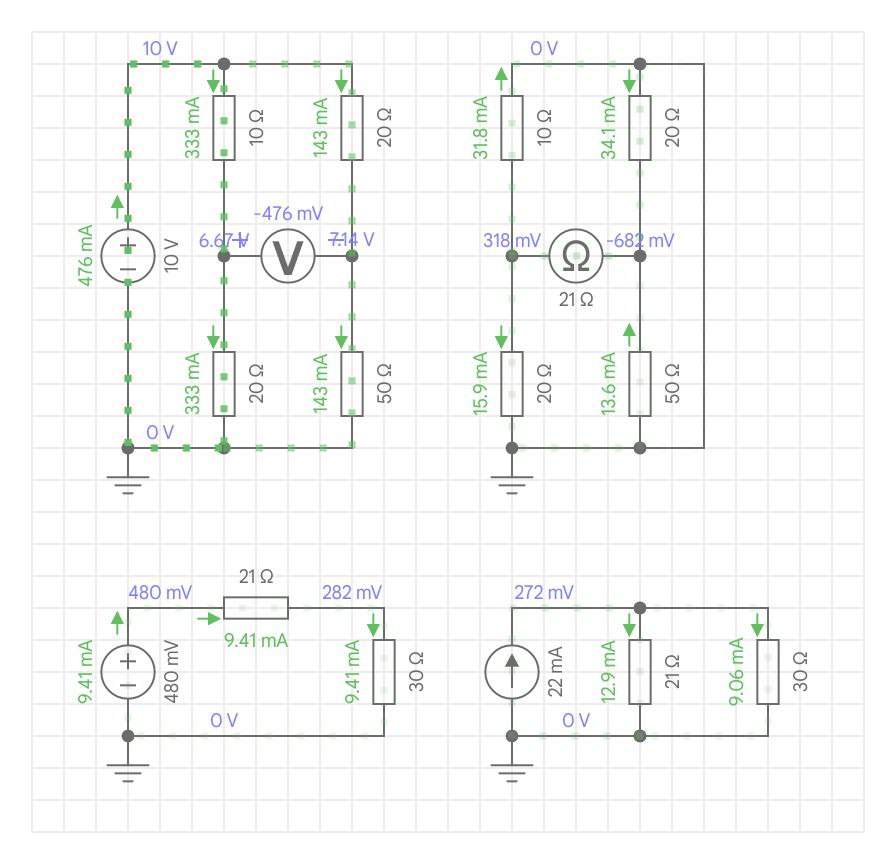
\includegraphics[width=.5\textwidth]{fig1}
	\caption{\textbf{CH1}}

	\columnbreak

	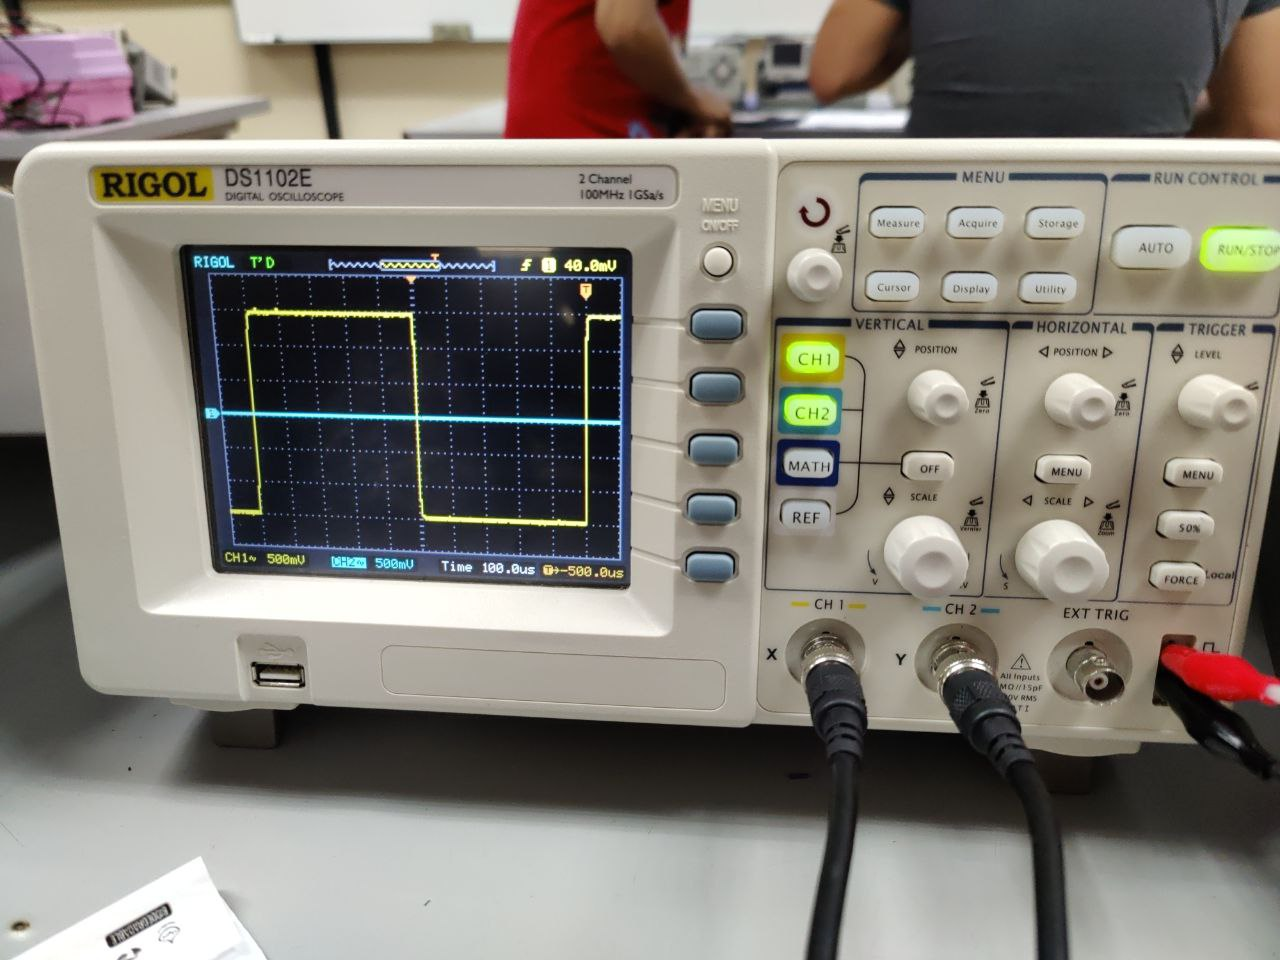
\includegraphics[width=.5\textwidth]{fig2}
	\caption{\textbf{CH2}}

	\end{multicols}
\end{figure}

\newpage

De modo que se obtuvo la siguiente información:

\begin{multicols}{2}

\begin{center} Canal 1 \end{center}

\emph{Time/Div} = $\SI{10}{\milli\second}$ \emph{Seg/Div} \\
\emph{Volts/Div} = $\SI{500}{\milli\volt}$ \emph{Volts/Div}\\

Con un periodo de

\[T_1 = 10 \times \SI{10}{\milli\second} = \SI{1}{\milli\second}\]

Así, la frecuencia se obtiene:

\[F_1 = \frac{1}{T} = \frac{1}{\SI{1}{\milli\second}} = \SI{1000}{\Hz}\]

Y para el valor del voltaje:

\[V_1 = \SI{500}{\milli\volt} \times 6 = 3 V_{pp}\]

\columnbreak

\begin{center} Canal 2 \end{center}
\emph{Time/Div} = $\SI{10}{\milli\second}$ \emph{Seg/Div} \\
\emph{Volts/Div} = $\SI{500}{\milli\volt}$ \emph{Volts/Div}\\

Así

\[T_2 = 10 \times \SI{10}{\milli\second} = \SI{1}{\milli\second}\]

Luego:

\[F_2 = \frac{1}{T} = \frac{1}{\SI{1}{\milli\second}} = \SI{1000}{\Hz}\]

Finalmente:

\[V_2 = \SI{500}{\milli\volt} \times 6 = 3 V_{pp}\]

\end{multicols}



\subsection{Comprobación del funcionamiento del generador de señales}

\subsubsection{Generación de señales}

Primero, se energizó el generador de señales, se conectó la terminal de salida a la entrada del \emph{canal 1} del osciloscopio con un cable conector \textbf{BNC-BNC}. Después, se ajustó la señal de salida del generador a $\SI{10}{\kHz}$ con una amplitud de $10V_{pp}$ y se comprobaron los diferentes tipos de señales que entregaba el generador.

\vspace{.5cm}

\begin{figure}[h!]
	\begin{multicols}{3}
	\centering

		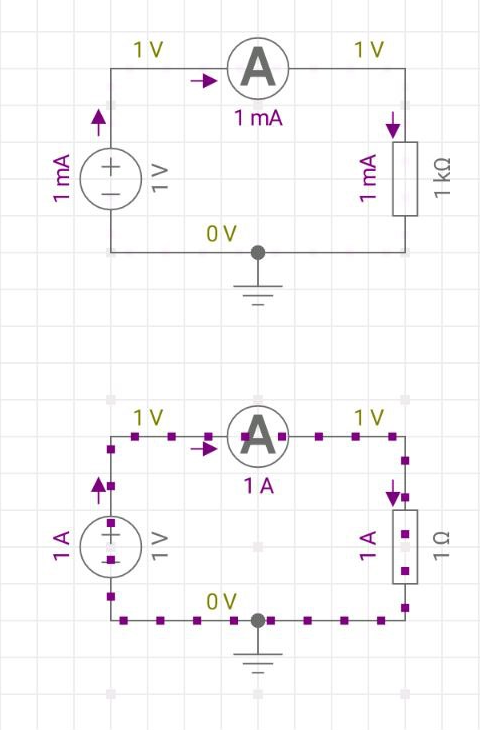
\includegraphics[width=.3\textwidth]{fig3}
		\caption{\textbf{Senoidal}}

	\columnbreak

		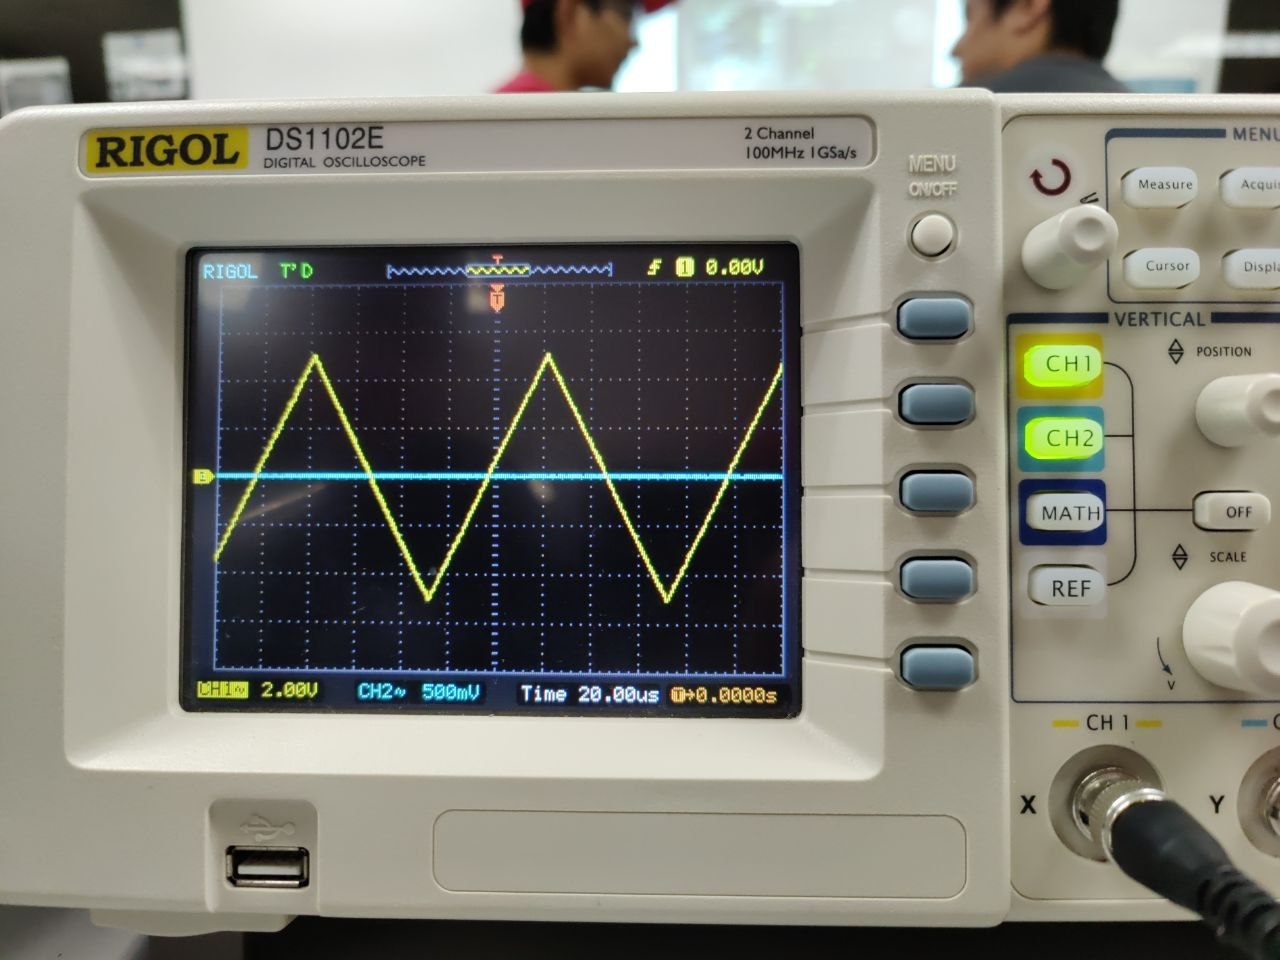
\includegraphics[width=.3\textwidth]{fig4}
		\caption{\textbf{Triangular}}

	\columnbreak

		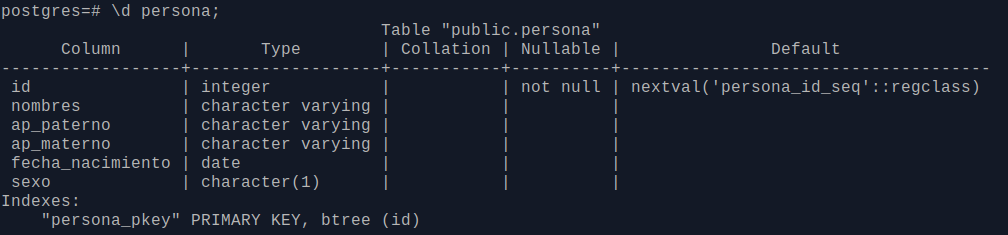
\includegraphics[width=.3\textwidth]{fig5}
		\caption{\textbf{Cuadrada}}


	\end{multicols}
\end{figure}

Como sólo se cambió el tipo de señal, tenemos la siguiente información sobre las características de las señales generadas:



\begin{center}
	\textbf{Amplitud $V_{pp}$} \emph{(Volts)}  = $\SI{10}{\volt}$ \\
	\textbf{Periodo $T$} \emph{(Seg)}  = $\SI{0.1}{\milli\second}$ \\
	\textbf{Frecuencia $F$} \emph{(Hz)}  = $\SI{10}{\kHz}$
\end{center}

\newpage

\subsubsection{Voltaje de \emph{OFFSET}}

En el generador de señales se seleccionó una señal triangular con $5 V_{pp}$ a una frecuencia de $\SI{10}{\kHz}$ y se conectó a la entrada del canal 1 del osciloscopio con una \emph{posición de acoplamiento} en \textbf{GND} con la traza en el centro de la gratícula del osciloscopio. Después, se cambió la posición de acoplamiento a \textbf{CD}, y en el generador se activó la generación de voltaje de \textbf{OFFSET} hasta valores máximos y mínimos, de modo que se ilustra en las figuras 7 y 8 los resultados:

\begin{figure}[h!]
	\centering
	\begin{multicols}{2}

	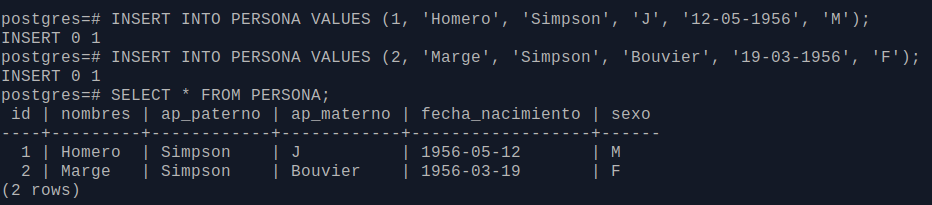
\includegraphics[width=.45\textwidth]{fig6}
	\caption{\textbf{OFFSET}$_{max} = \SI{7}{\volt}$}

	\columnbreak

	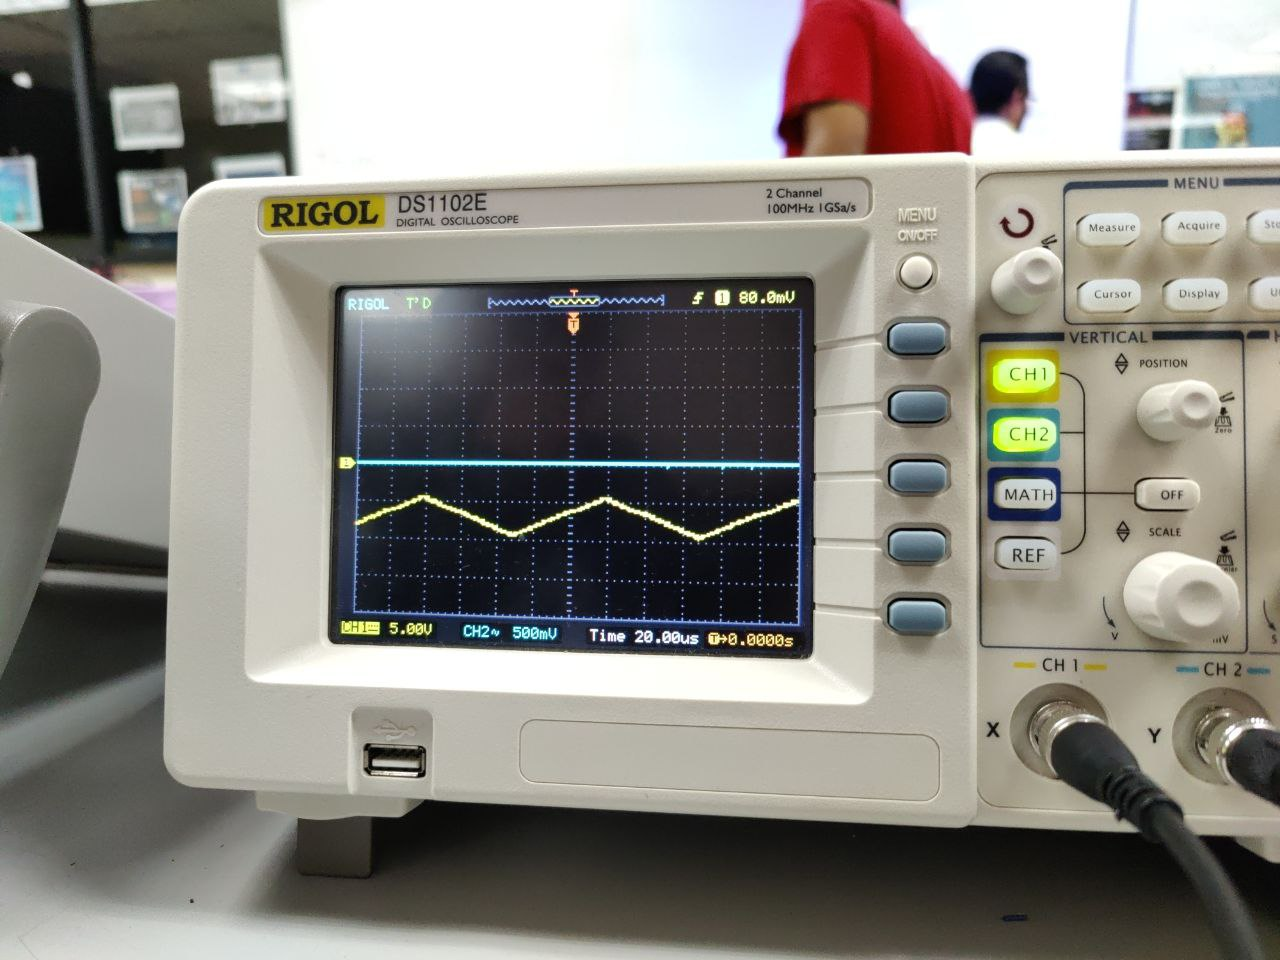
\includegraphics[width=.45\textwidth]{fig7}
	\caption{\textbf{OFFSET}$_{min} = -\SI{7}{\volt}$}

	\end{multicols}
\end{figure}

\vspace{-0.5cm}

\subsection{El osciloscopio como graficador X-Y con señales de CD}

Se midió el desplazamiento cartesiano del haz electrónico sujeto a distintas polaridades de tensión de CD en las terminales de entrada del osciloscopio.\\
Primero, se colocó el osciloscopio en modo \textbf{X-Y} con los selectores de acoplamiento de ambos canales en la posición \textbf{GND}. Se emplearon los controles de \emph{posición X} y \emph{posición X} para colocar los trazos de ambos canales en el centro (u origen), de manera que el punto se encontrara en el centro de la pantalla del osciloscopio.\\
Después se construyó el Circuito 1 de la Figura 9 y se realizaron las mediciones en los puntos \textbf{A, B y C} según las indicaciones:\\



\begin{figure}[h!]
	\centering
	  \begin{circuitikz}[american, voltage dir=RP] 
	  		\path (6,6) node[anchor=west](A){$A$};
			\path (6,3) node[anchor=west](B){$B$};
			\path (6,0) node[anchor=west](C){$C$};
			\draw	(0,0) 
	  		to[battery, l=$E$, a=$\SI{10}{\volt}$] (0,6) -- (4,6)
			to[R, a=$R_1$, l=$\SI{10}{\kohm}$,*-] (4,3)
			to[R, a=$R_2$, l=$\SI{10}{\kohm}$,*-*] (4,0) -- (0,0);
			\draw (4,6) to[short,-*] (6,6);
			\draw (4,3) to[short,-*] (6,3);
			\draw (4,0) to[short,-*] (6,0);
		\end{circuitikz}
		\caption{Circuito 1}
\end{figure}


\begin{enumerate}

\item	Positivo del canal X al punto \textbf{A}, y negativo del canal X al punto \textbf{C}.
\begin{figure}[h!]
\centering
	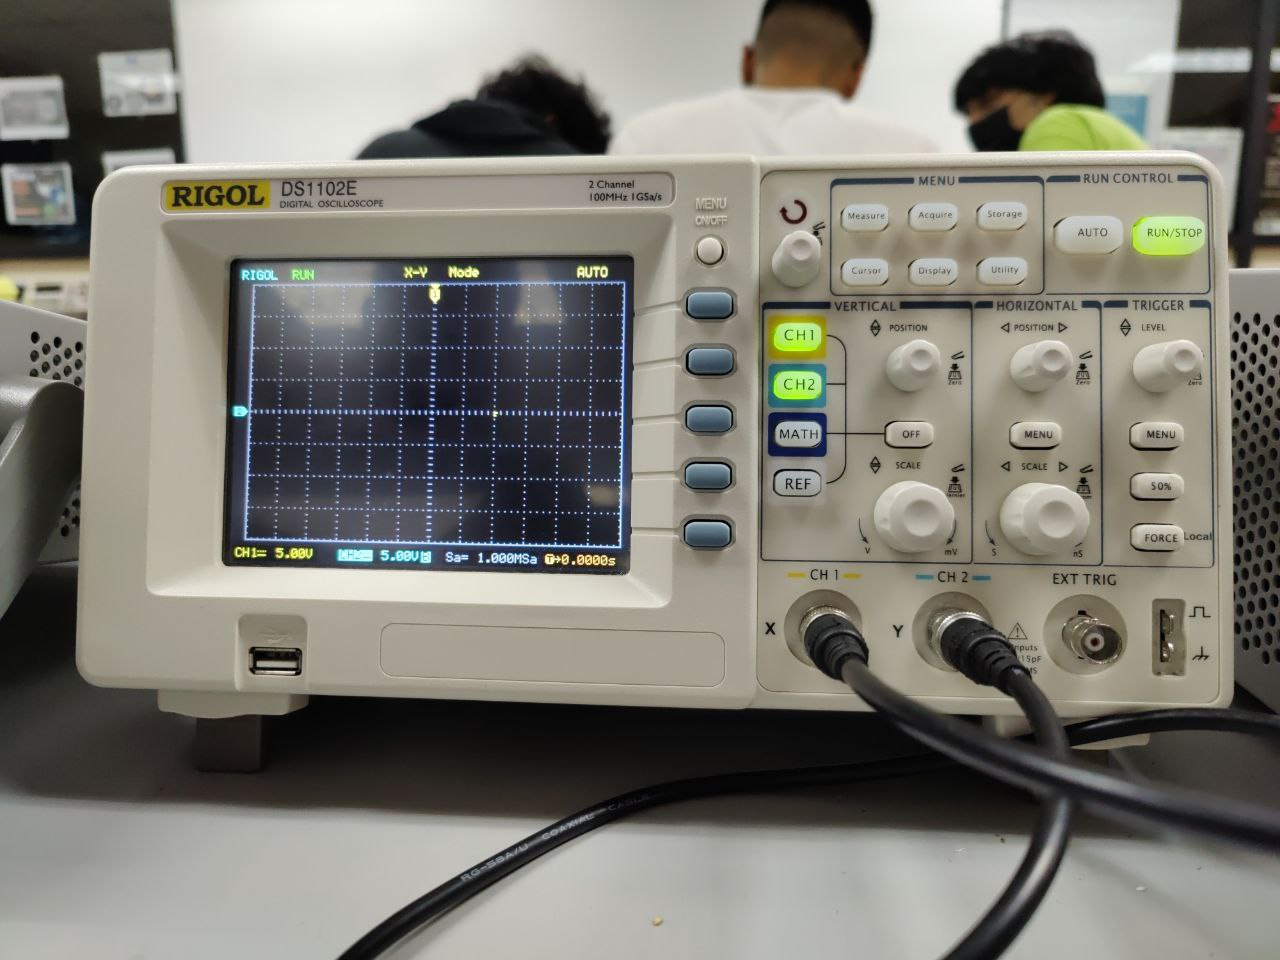
\includegraphics[width=.45\textwidth]{fig8}
	\caption{Coordenadas: $(2,0)$}
\end{figure}

\item	Positivo del canal Y al punto \textbf{B}, y negativo del canal Y al punto \textbf{C}.
\begin{figure}[h!]
\centering
	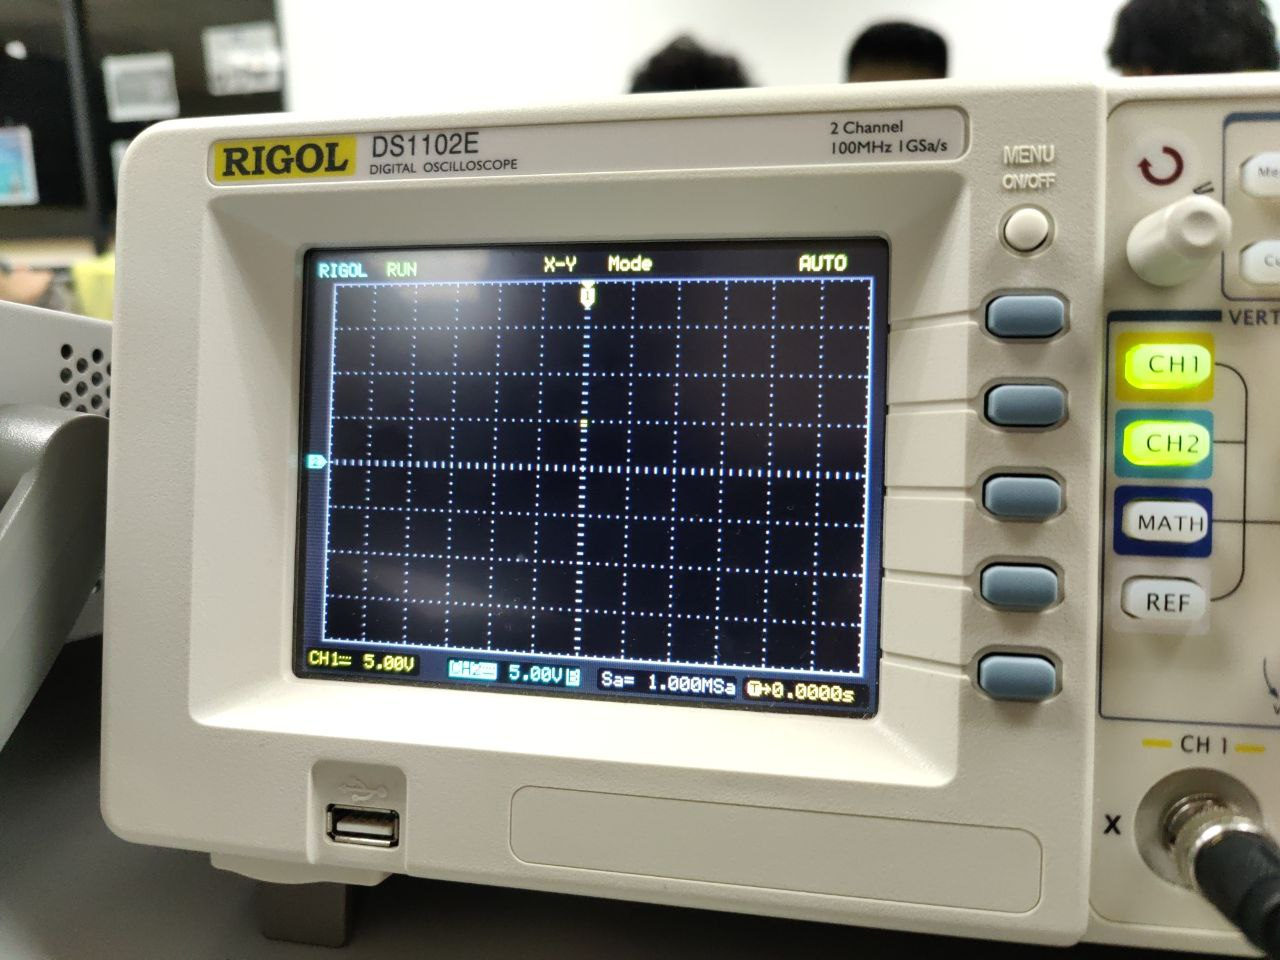
\includegraphics[width=.45\textwidth]{fig9}
	\caption{Coordenadas: $(0,1)$}
\end{figure}

\item	Positivo del canal X al punto \textbf{A}, positivo del canal Y al punto \textbf{B}, y negativos de ambos canales al punto \textbf{C}.
\begin{figure}[h!]
\centering
	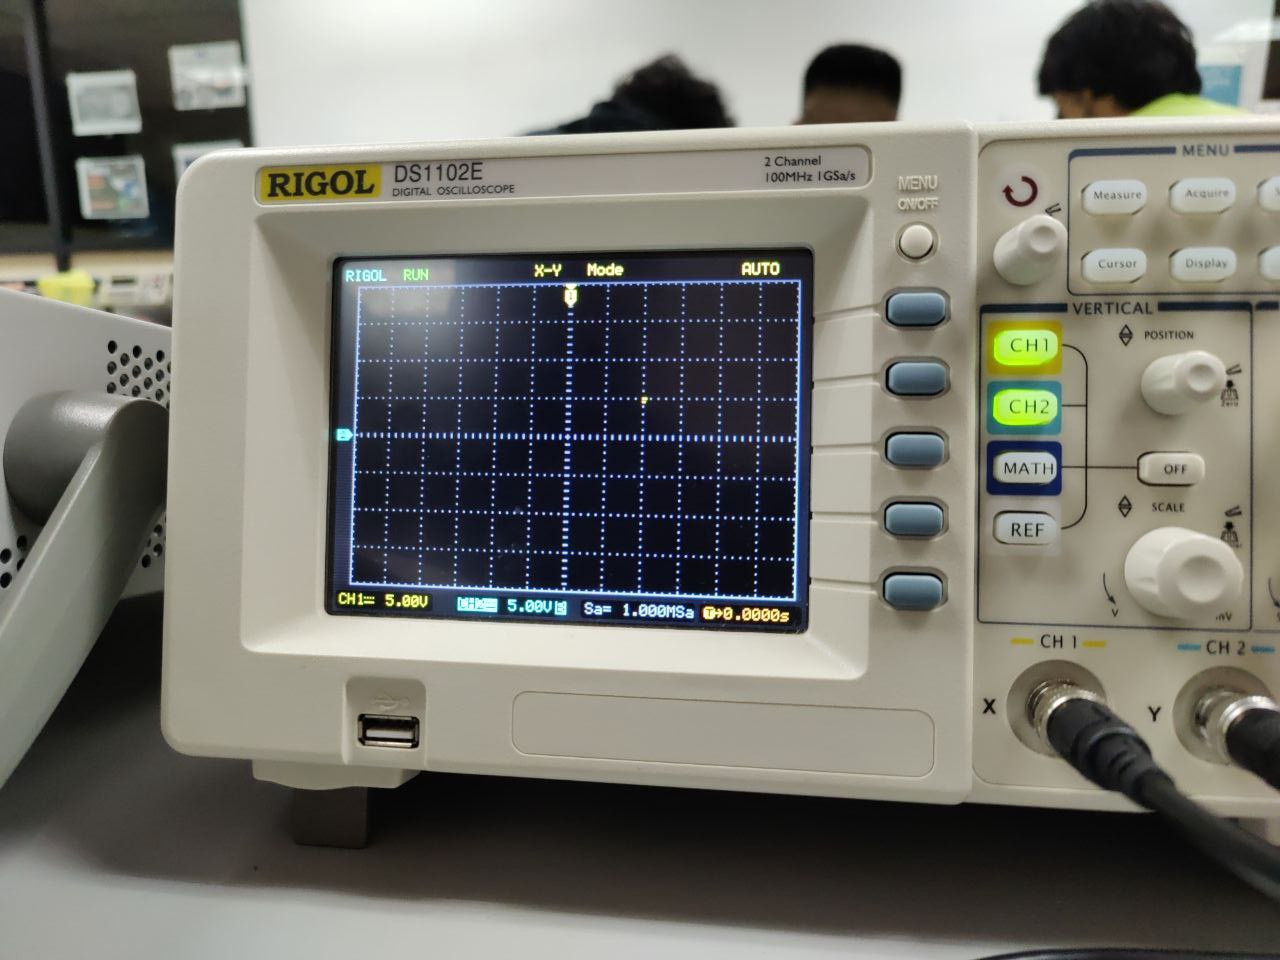
\includegraphics[width=.45\textwidth]{fig10}
	\caption{Coordenadas: $(2,1)$}
\end{figure}

\newpage

\item	Misma conexión del punto anterior pero con el canal Y invertido.
\begin{figure}[h!]
\centering
	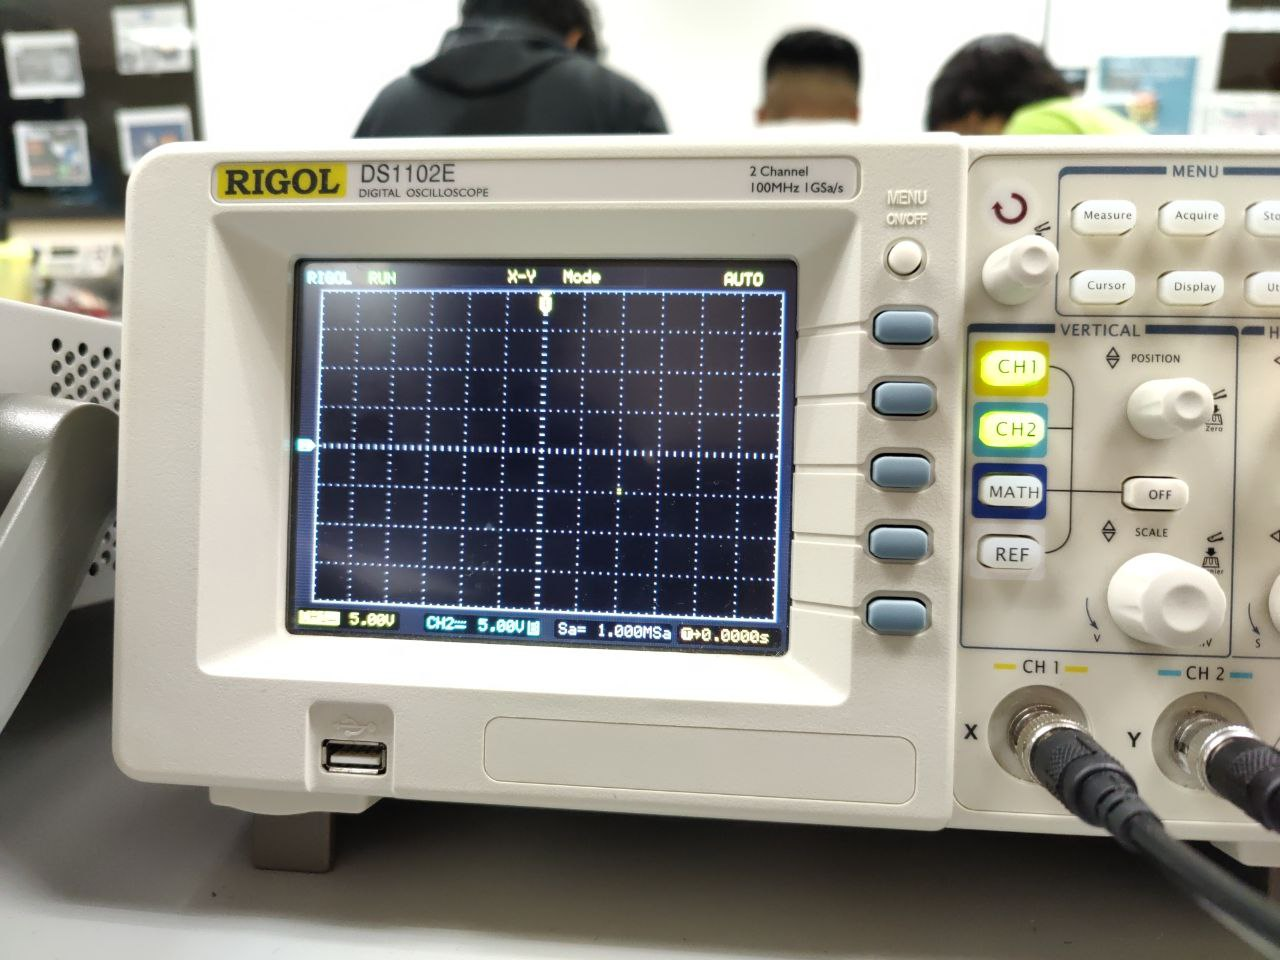
\includegraphics[width=.45\textwidth]{fig11}
	\caption{Coordenadas: $(2,-1)$}
\end{figure}

\item	Positivo del canal X al punto \textbf{B}, positivo del canal Y al punto \textbf{C}, y negativos de ambos canales al punto \textbf{A} y canal Y invertido.
\begin{figure}[h!]
\centering
	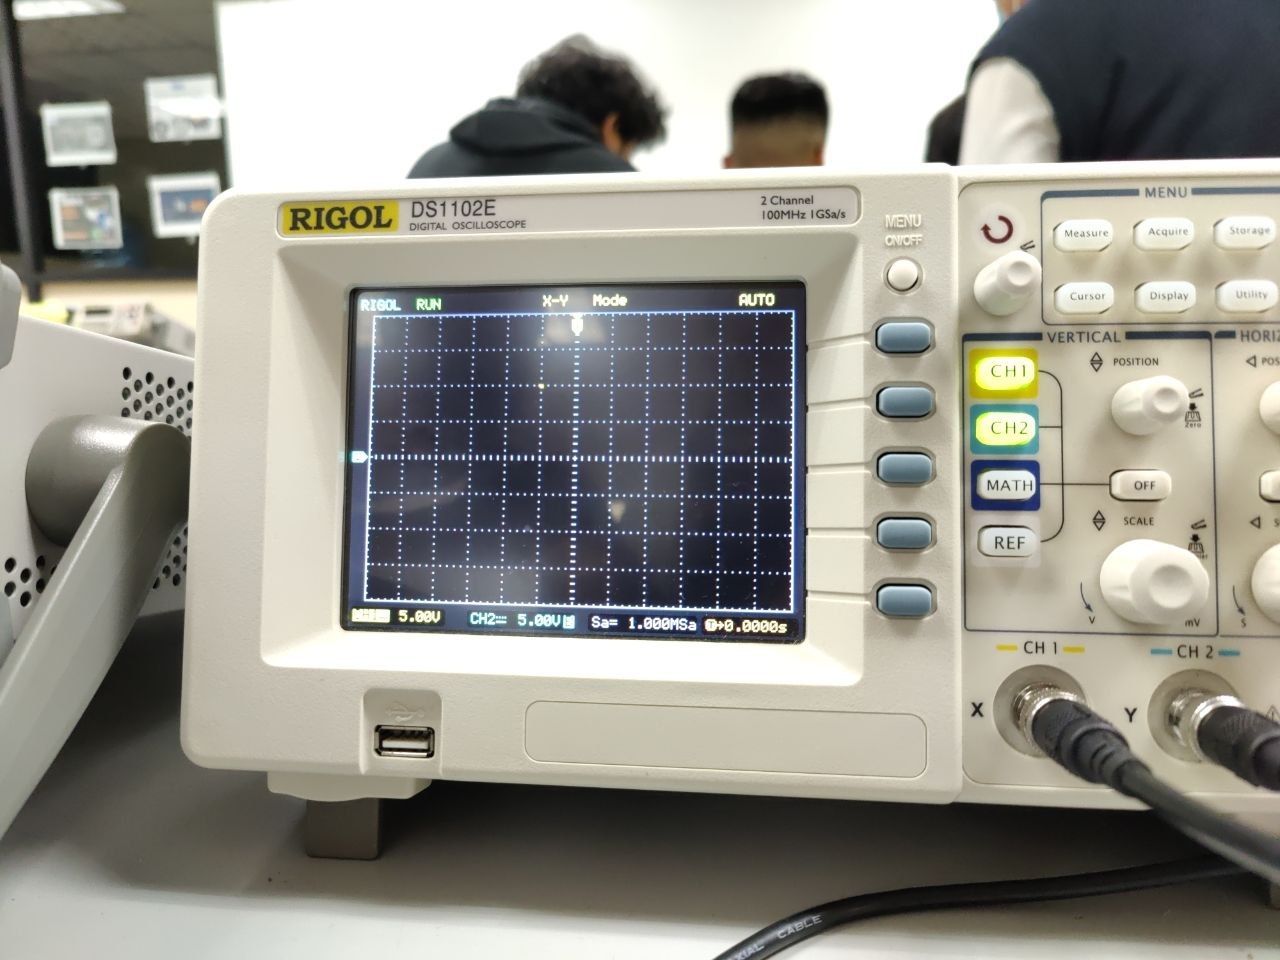
\includegraphics[width=.45\textwidth]{fig12}
	\caption{Coordenadas: $(-1,2)$}
\end{figure}

\end{enumerate}


\subsection{El osciloscopio como graficador X-Y con señales de CA}

Del Circuito 2 de la Figura 15 se midió el ángulo de desfasamiento utilizando al osciloscopio como graficador respecto al tiempo \textbf{Y(t)} y como \textbf{XY} (método \emph{Lissajous}):


\begin{figure}[h!]
	\centering
	  \begin{circuitikz}[american, voltage dir=RP] 
	  		\path (6,4.5) node[anchor=west](X){$X$};
			\path (6,3) node[anchor=west](Y){$Y$};
			\path (6,0) node[anchor=west](T){$T$};
			\draw	(0,0) 
	  		to[sV=$12V_{pp}$, a=$\SI{300}{\Hz}$] (0,3)
			to[C, a=$C$, l=$\SI{0.1}{\micro\farad}$,*-*] (4,3)
			to[R, a=$R$, l=$\SI{4.7}{\kohm}$,-*] (4,0) -- (0,0);
			\draw (0,3) to[short] (0,4.5) to [short, -*] (6,4.55);
			\draw (4,3) to[short,-*] (6,3);
			\draw (4,0) to[short,-*] (6,0);
		\end{circuitikz}
		\caption{Circuito 2}
\end{figure}

Para ambos modos se utilizó:\\

\begin{center}
	\emph{Volts/Div} = $\SI{2}{\volt}$\\
	\emph{Time/Div} = $\SI{1}{\milli\second}$\\
\end{center}

\newpage

De donde, para calcular el ángulo de desfasamiento $\phi$ en el modo \textbf{Y(t)}, siendo $a = 0.4$ la diferencia respecto al tiempo entre ambas señales producido por el capacitor, se tiene:

\vspace{0.3cm}

\begin{figure}[h!]
	\centering
	\begin{multicols}{2}

	\[ \phi = \frac{360\degree (\SI{0.4}{\milli\second}) }{\SI{3.4}{\milli\second}} = 42.35\degree\]

	\columnbreak

	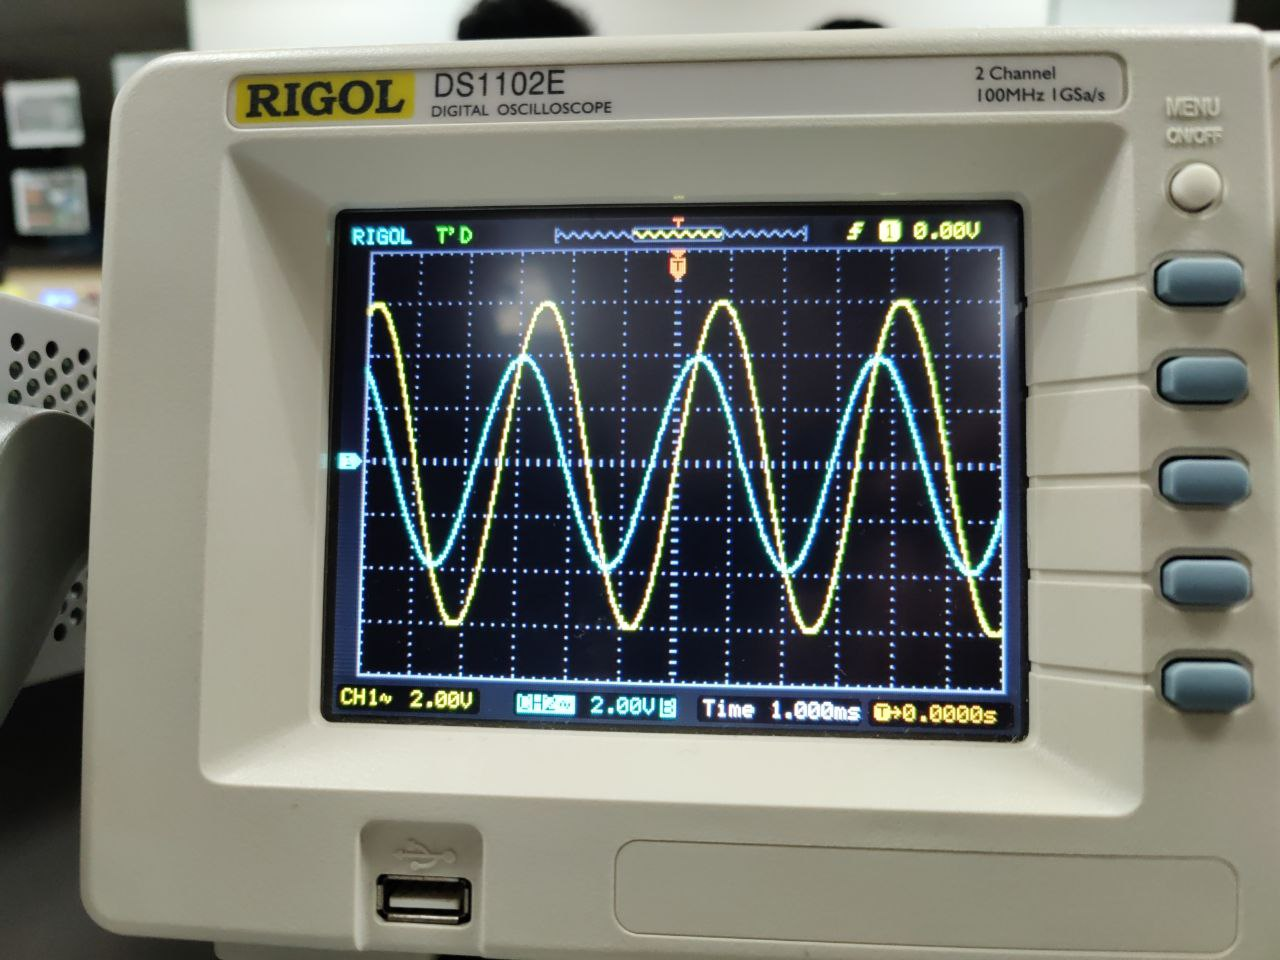
\includegraphics[width=.5\textwidth]{fig13}
	\caption{\textbf{Y(t)}}
	
	\end{multicols}
\end{figure}

Y para el modo \textbf{XY} con $A = \SI{2}{\milli\second}$ y $B = \SI{1.3}{\milli\second}$ tenemos:

\begin{figure}[h!]
	\centering
	\begin{multicols}{2}


	\[\phi = \arcsen(\dfrac{\SI{1.3}{\milli\second}}{\SI{2}{\milli\second}}) \approx 40.54\degree \] \\
	Con $A = \SI{1.9}{\milli\second}$
	\[\phi = \arcsen(\dfrac{\SI{1.4}{\milli\second}}{\SI{1.9}{\milli\second}}) \approx 43.17\degree \]


	\columnbreak

	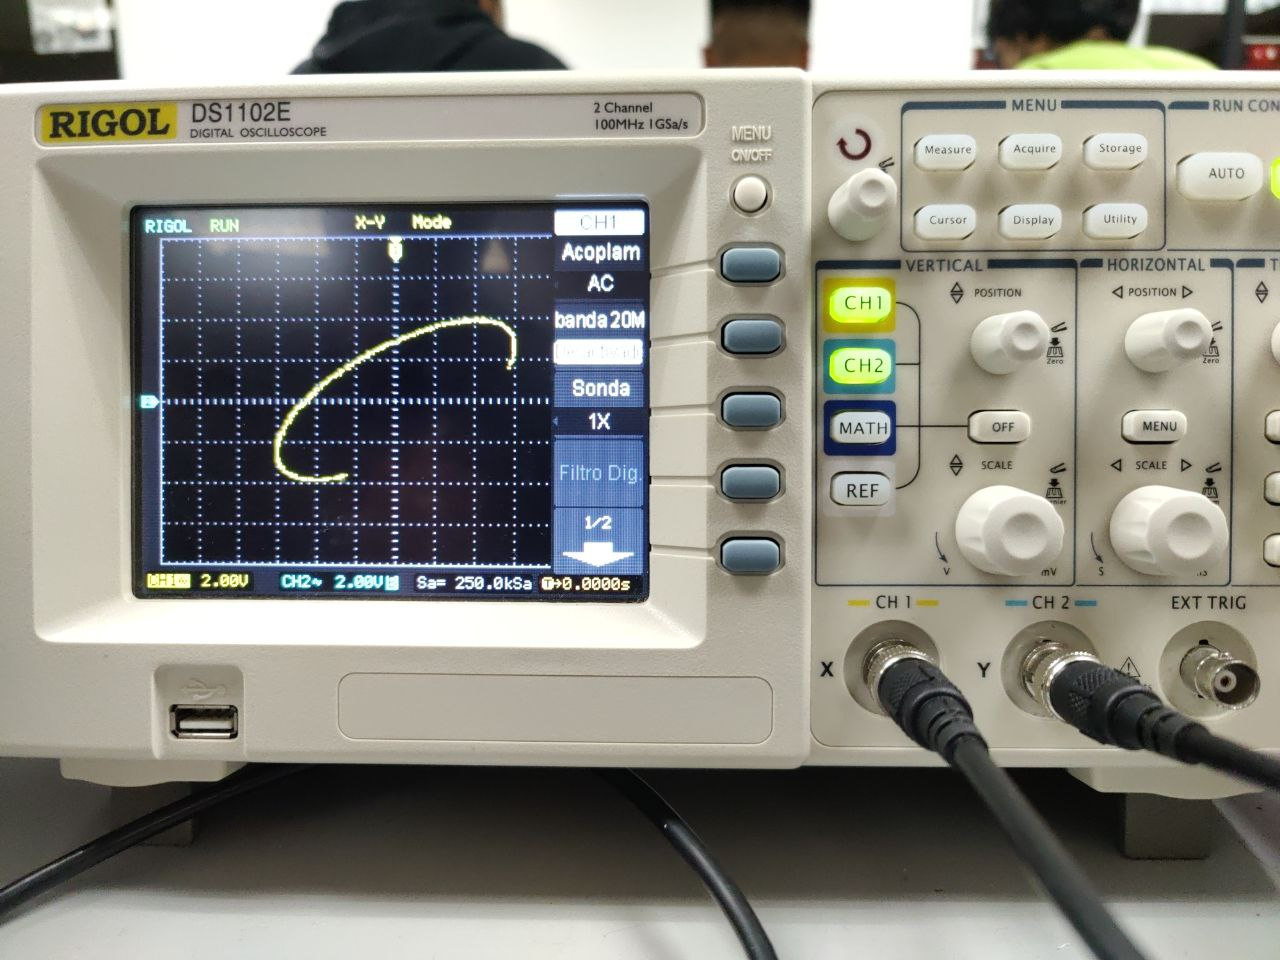
\includegraphics[width=.5\textwidth]{fig14}
	\caption{\textbf{XY} (método \emph{Lissajous})}

	\end{multicols}
\end{figure}



\newpage

\section{Cuestionario}

\vspace{0.5cm}

\begin{enumerate}

	\item Explique el funcionamiento del \emph{osciloscopio}:
	Un osciloscopio es un instrumento de medición utilizado en el campo de la electrónica de señal el cual representa en un gráfico las diferentes señales eléctricas que tienen la capacidad de poder variar en el tiempo. Los osciloscopios comprueban y muestran las señales de tensión como formas de onda y como representaciones visuales de la variación de tensión en función del tiempo

	\item ¿Cuál es la función de un generador de señales? \\ Un generador de señales es un dispositivo electrónico que produce una señal de voltaje alterno con características específicas, como frecuencia, amplitud y forma de onda, y se utilizan en distintas aplicaciones de prueba y medición, como calibración de instrumentos de medida, pruebas de circuitos electrónicos y comunicaciones.
	
	\item ¿Para qué sirven las gráficas de \emph{Lissajous}? \\ Las gráficas de Lissajous se emplean para determinar la frecuencia y fase relativa entre dos oscilaciones senoidales. Las gráficas de Lissajous se obtienen por la superposición de dos oscilaciones armónicas en direcciones perpendiculares entre ellas (90°) 1. El movimiento resultante depende sensiblemente de los parámetros de cada oscilación: Amplitud, frecuencia y fase.
	
	\item ¿Para qué se emplean los modos de funcionamiento \textbf{Y(t)} y \textbf{XY}? \\ Para mostrar las diferentes señales que se miden con un osciloscopio como funciones de tiempo (Y(t)) o una función entre dos canales de medición (XY).
	
	\item ¿Qué entiende por acoplamiento en DC? \\ Que la información que proyecta el osciloscopio se muestra como un valor de corriente directa, es decir, sin la parte negativa de una señal de corriente alterna.
	
	\item ¿Qué es una señal de \emph{OFFSET}? \\ Una señal de \emph{OFFSET} se puede definir como el nivel de corriente continua que le suma a una señal alterna. Así, si la señal está centrada en el origen, se dice que el nivel de \emph{offset} es 0. Si está desplazada hacia arriba, el \emph{offset} es positivo, mientras que si está desplazada hacia abajo, será negativo.
	
	\item ¿Qué significa que una señal se encuentre desfasada? \\ Entre dos señales que tienen el mismo periodo, una se encuentra desfasamiento respecto a otra si sus magnitudes no son simultáneas, es decir, una alcanza el valor máximo o mínimo de su amplitud antes o después que la otra, considerándose adelantada o atrasada, y teniendo un ángulo de desfase.

\end{enumerate}

\newpage

\section{Conclusiones}

\vspace{.5cm}

{\Large González Cárdenas Ángel Aquilez}\\

\vspace{.3cm}

Tras concluir la práctica, se ajustaron correctamente las señales de calibración para los canales 1 y 2 de manera que nos permitió observar un ciclo completo de la señal cuadrada de calibración. Luego, se comprobó el correcto funcionamiento del generador de señales al producir una señal y variando su forma entre triangular, cuadrada y senoidal. Después se graficaron dos señales de corriente directa con el modo \emph{XY}, obteniendo un punto de luz a través del plano cartesiano del osciloscopio e invertido los diferentes canales para desplazar el punto. También se comprobó la función de OFFSET del generador de funciones para desplazar de manera vertical una señal con un valor mínimo y máximo. Finalmente, se visualizó el desfase entre dos señales por la interacción de la corriente generada por el capacitor de un circuito y como el almacenamiento de carga provoca el desfase en un circuito. Cabe mencionar que el modo \emph{XY} con corriente directa solo arrojó un punto de luz, mientras que en corriente alterna trazó una elipse.

\vspace{1cm}

{\Large Sánchez González Daniel Iván}\\
\vspace{.3cm}

Tras ajustar adecuadamente las señales de calibración para ambos canales, se visualizó un ciclo completo de la señal cuadrada de calibración en ambos canales respectivamente. Además, se verificó que el generador de señales funcionara correctamente al generar una señal y cambiar su forma entre tres tipos distintos: triangular, cuadrada y senoidal. Posteriormente, se graficaron dos señales de corriente directa en modo \emph{XY}, lo que resultó en un punto de luz en el plano cartesiano del osciloscopio. Al tomar las mediciones en diferentes puntos del circuito e invertir los canales, se desplazó el punto a lo largo del plano cartesiano del osciloscopio pero sin alterarse las magnitudes correspondientes del voltaje. También se probó la función OFFSET del generador de funciones para desplazar verticalmente una señal con un valor mínimo y máximo, al percibirse un sonido de alerta que indicaba el alcance del valor máximo o mínimo. Finalmente, se observó el desfase entre dos señales debido a la interacción de la corriente por el capacitor entre los modos \emph{Y(t)} y \emph{XY}.


\section{Bibliografía}

\begin{itemize}
\item Desfase. (s. f.). En Wikipedia. Recuperado el 18 de junio de 2023, de https://es.wikipedia.org/wiki/Desfase
\item Ejemplos.net. (s. f.). Que significa offset en electronica. Recuperado el 18 de junio de 2023, de https://ejemplos.net/que-significa-offset-en-electronica/
\item Soundcheck.com.mx. (2021, julio 1). DC Offset. Recuperado el 18 de junio de 2023, de https://soundcheck.com.mx/dc-offset-lo-que-siempre-quisiste-saber-y-nadie-te-supo-explicar/
\item Unidad de Apoyo Para el Aprendizaje - UNAM. (s. f.). Función senoidal, desfasamiento. Recuperado el 18 de junio de 2023, de
\end{itemize}

\newpage
\section{Anexos}
\subsection{Simulación del Circuito 1}

A continuación se presentan los resultados de las simulaciones de los circuitos de las figuras 9 y 15 para contrastarlos con las mediciones y cálculos realizados. Se generaron gracias a la aplicación multiplataforma \textit{EveryCircuit}\texttrademark. \\


\begin{figure}[!h]
\centering
	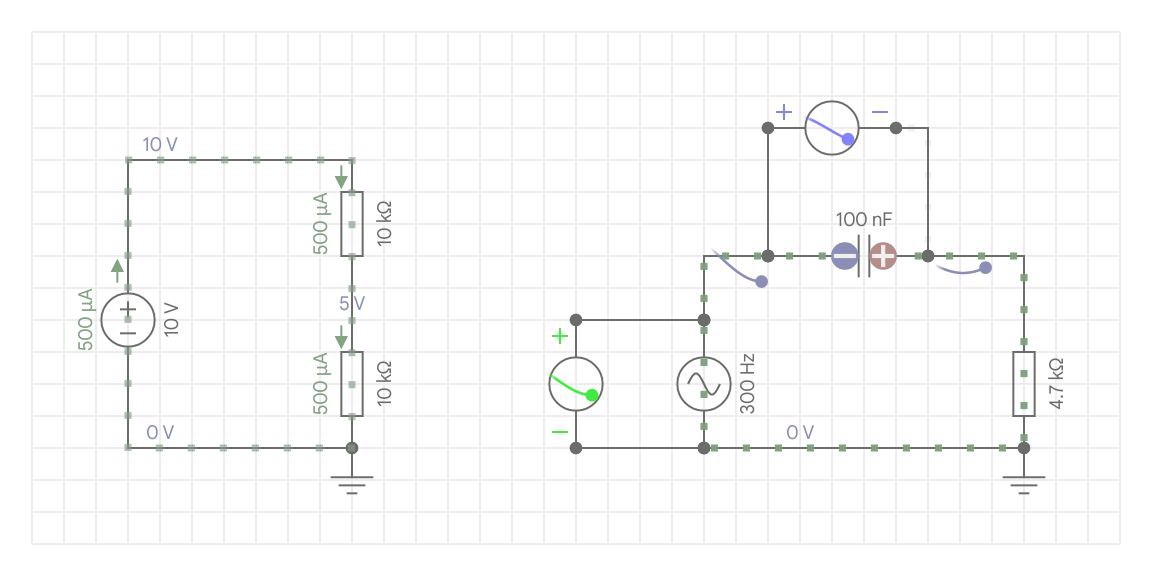
\includegraphics[width=.8\textwidth]{fig15}
	\caption{Simulación de los circuitos 1 y 2}
\end{figure}

\begin{figure}[!h]
\centering
	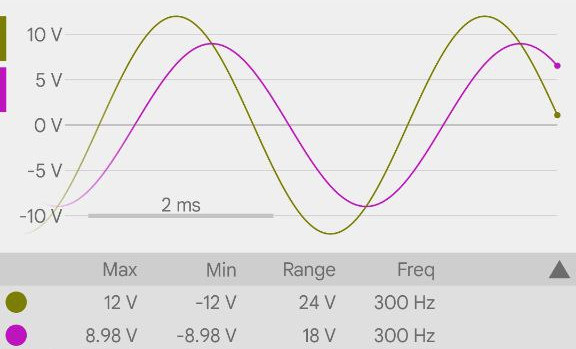
\includegraphics[width=.8\textwidth]{fig16}
	 \caption{Simulación del ángulo de desfasamiento}
\end{figure}


\end{document}